\makeatletter
\@openrightfalse
\makeatother

\chapter*{Přílohy}
\addcontentsline{toc}{chapter}{Přílohy}



%%\section*{Seznam příloh}
\noindent
\noindent
\textbf{A}~-- Schémata prototypu \dotfill \pageref{app:schematics}\\[2mm]
\textbf{B}~-- Vodivé motivy DPS \dotfill \pageref{app:pcb_layers}

\section*{Obsah elektronické přílohy}

\begin{enumerate}
	\item Návrhové soubory prvního prototypu (formát KiCAD 9.0)
	\item Návrhové soubory druhého prototypu (formát KiCAD 10.0)
	\item Firmware pro STM32F103C8
	\item PC aplikace -- zdrojový kód
\end{enumerate}

\newgeometry{hmargin=1.5cm, top=1.5cm, bottom=2cm, footskip=5mm}

\renewcommand{\thesection}{\Alph{section}}
\setcounter{section}{0}

\section{Schémata prototypu}
\label{app:schematics}

\begin{figure}[H]
    \centering
    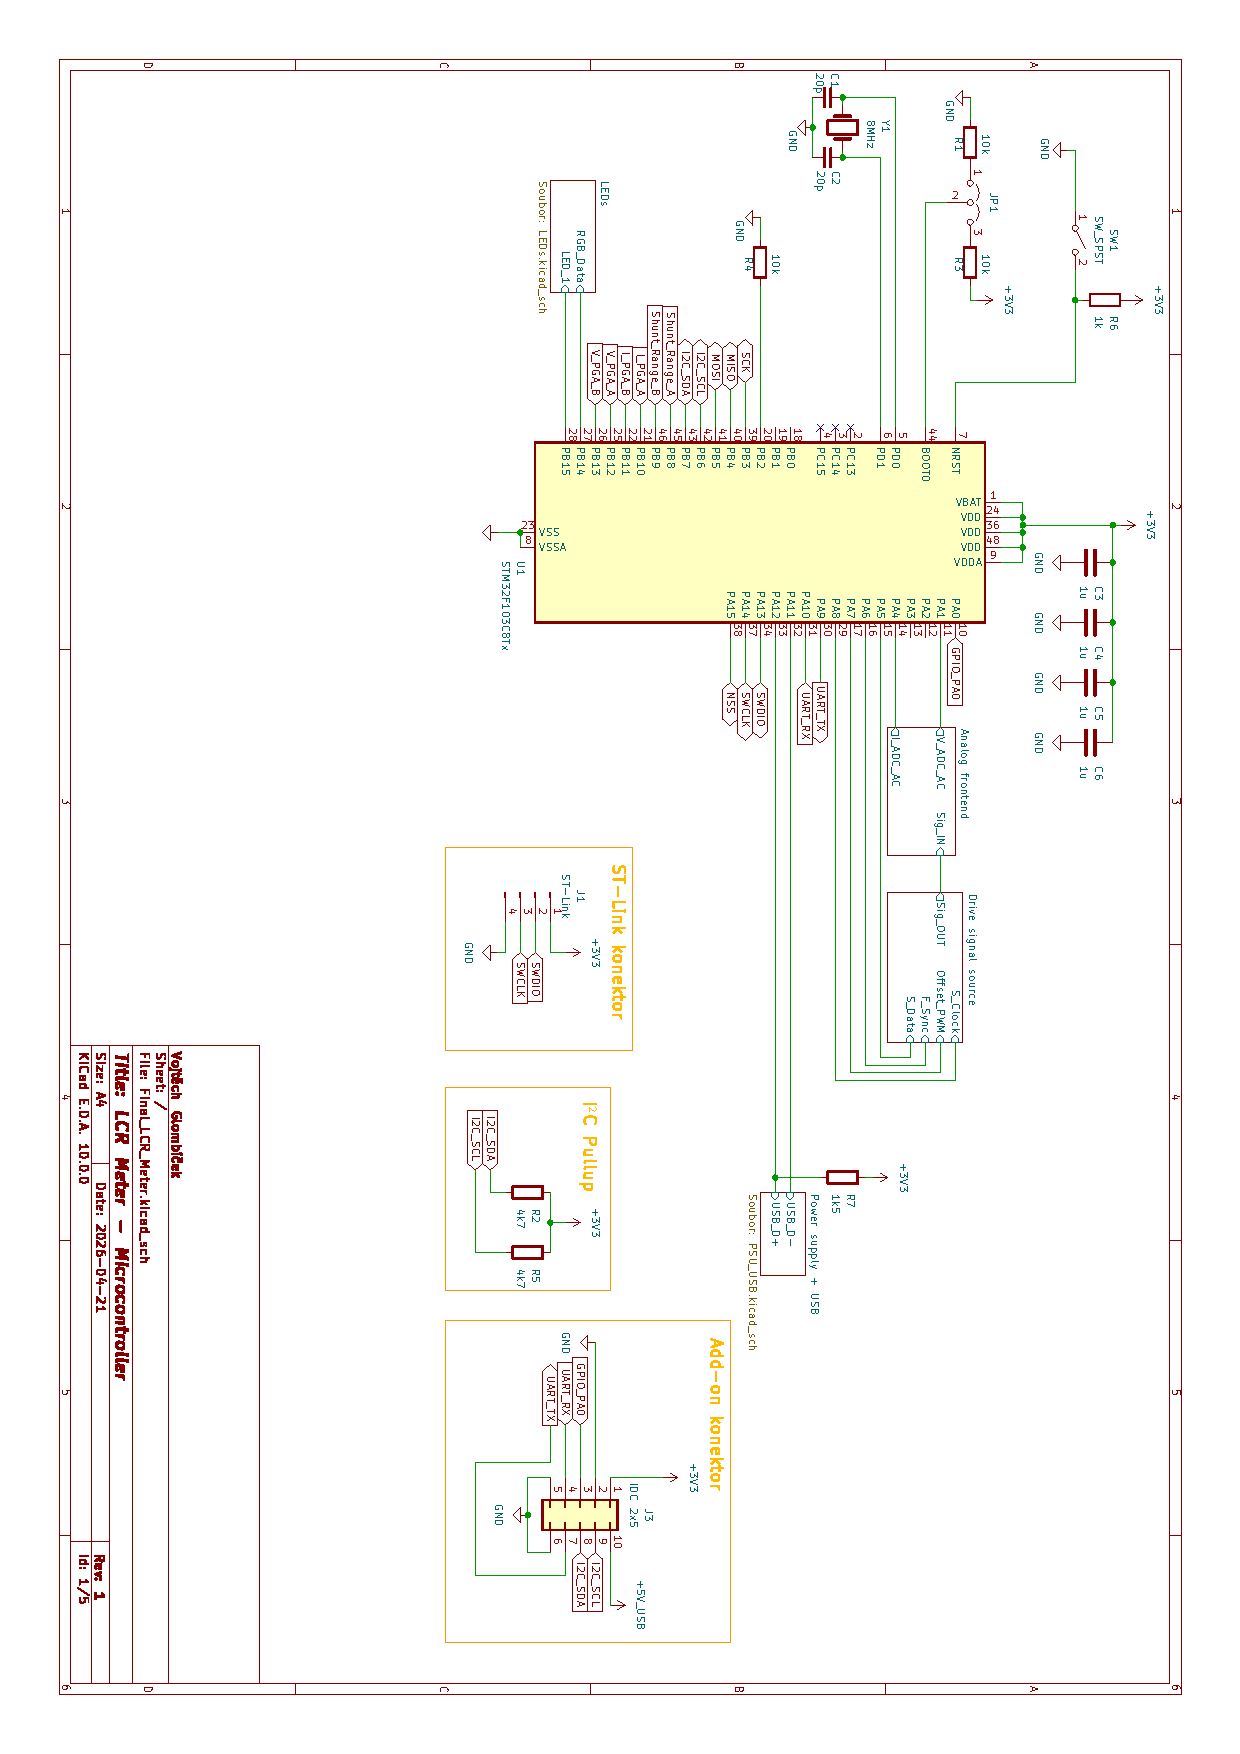
\includegraphics[width=\textwidth,height=\textheight,keepaspectratio]{obrazky/schema+layout/Final_LCR_Meter_page_1.pdf}
    \caption{Schéma -- strana 1 - mikrokontrolér}
\end{figure}

\begin{figure}[H]
    \centering
    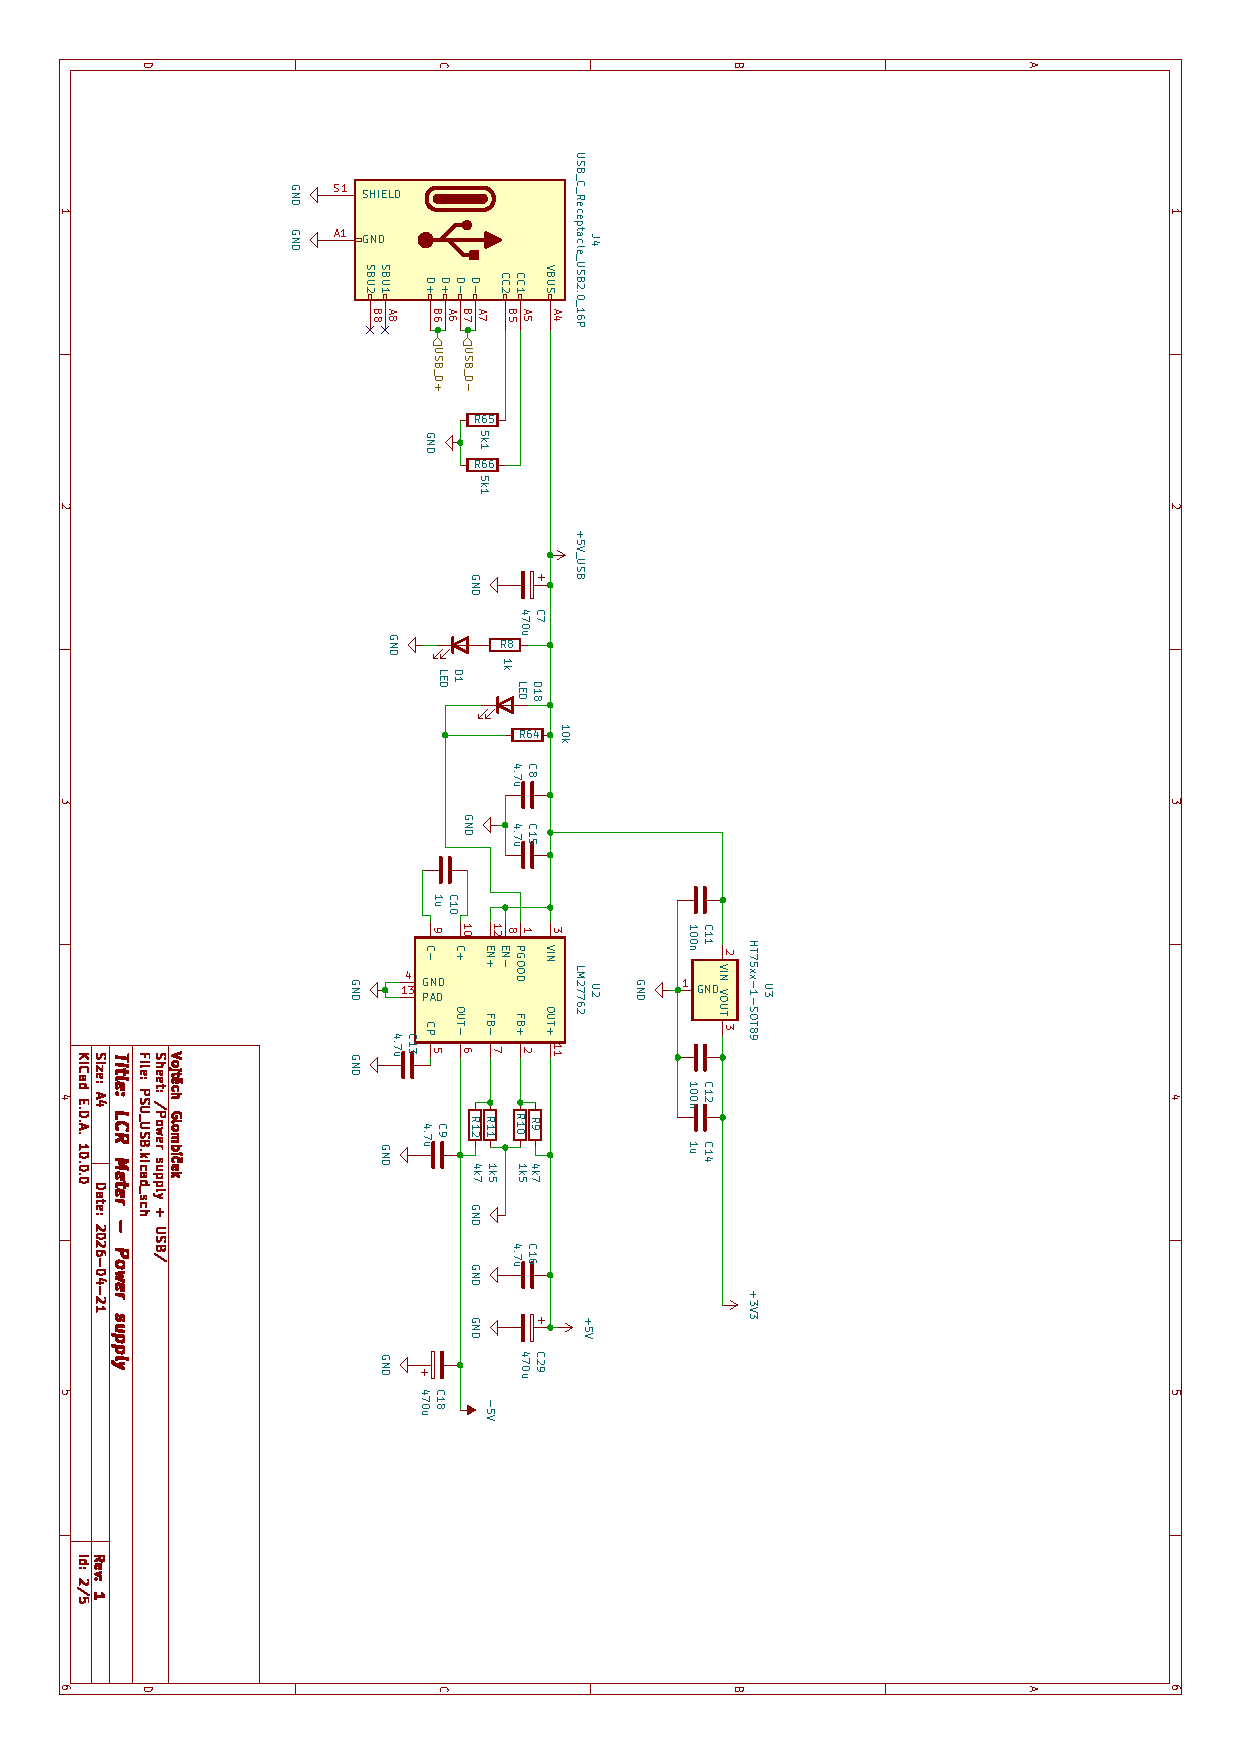
\includegraphics[width=\textwidth,height=\textheight,keepaspectratio]{obrazky/schema+layout/Final_LCR_Meter_page_2.pdf}
    \caption{Schéma -- strana 2 - napájení}
\end{figure}

\begin{figure}[H]
    \centering
    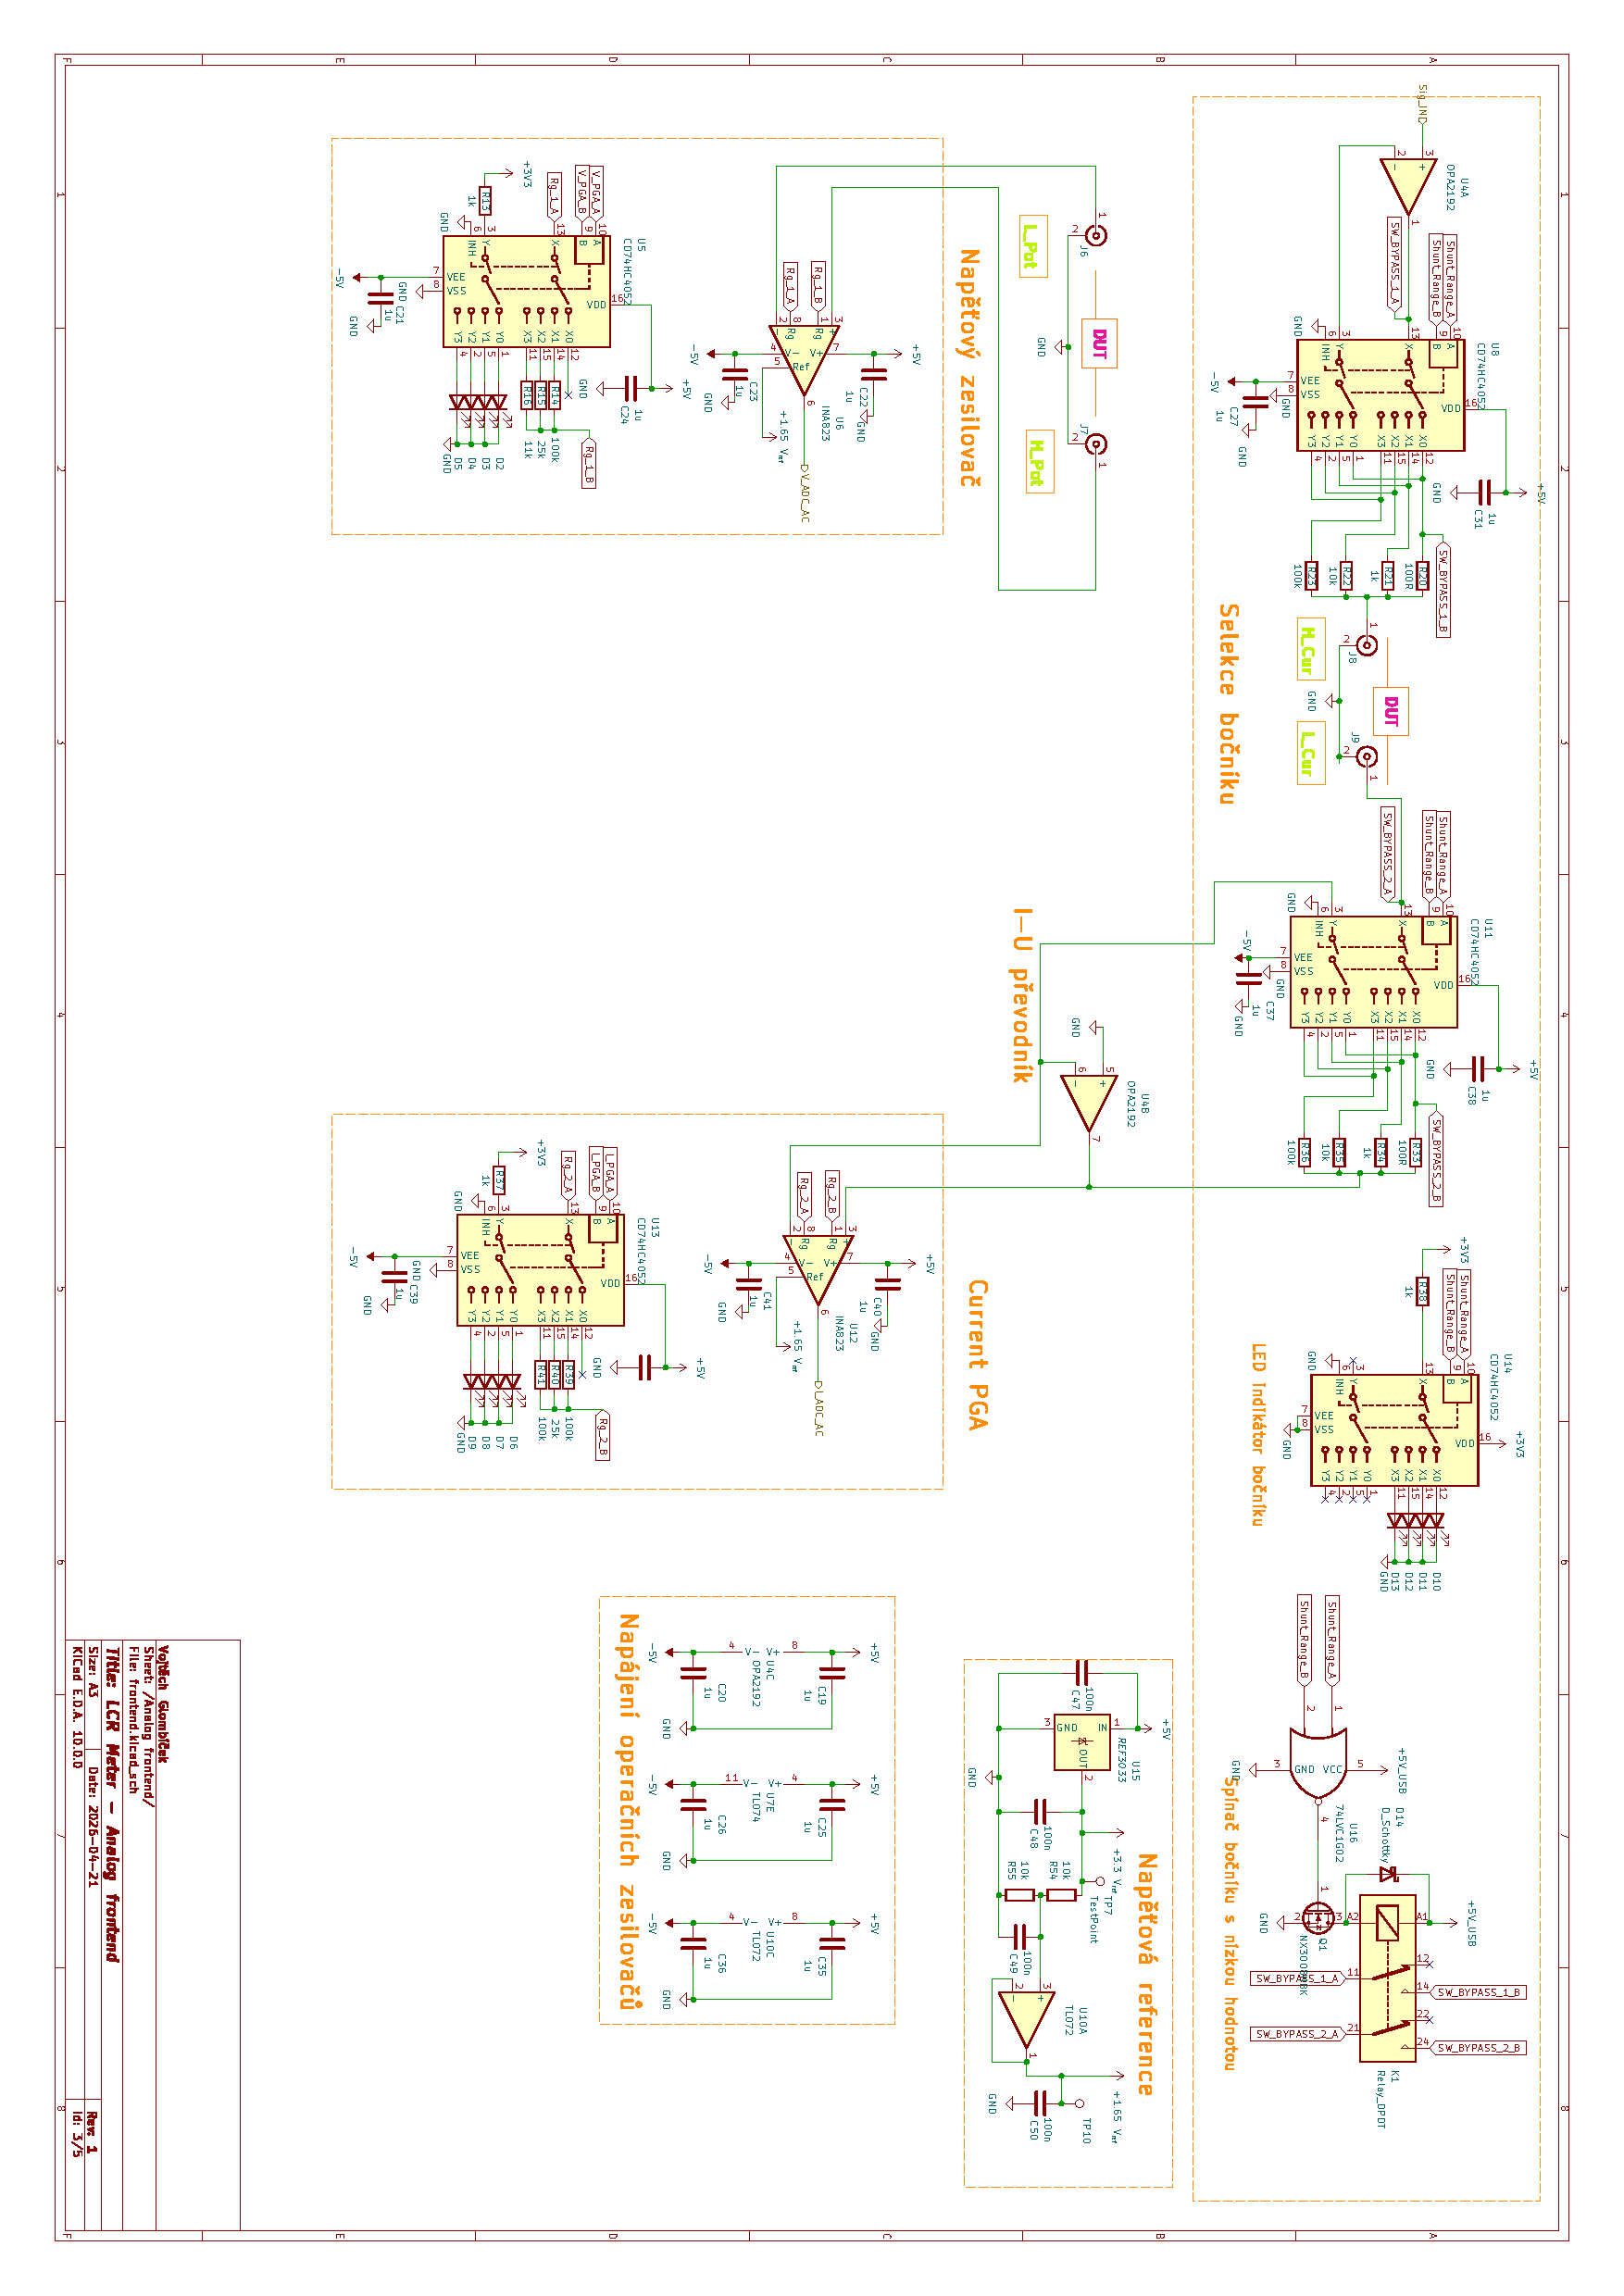
\includegraphics[width=\textwidth,height=\textheight,keepaspectratio]{obrazky/schema+layout/Final_LCR_Meter_page_3.pdf}
    \caption{Schéma -- strana 3 - analogový frontend}
\end{figure}

\begin{figure}[H]
    \centering
    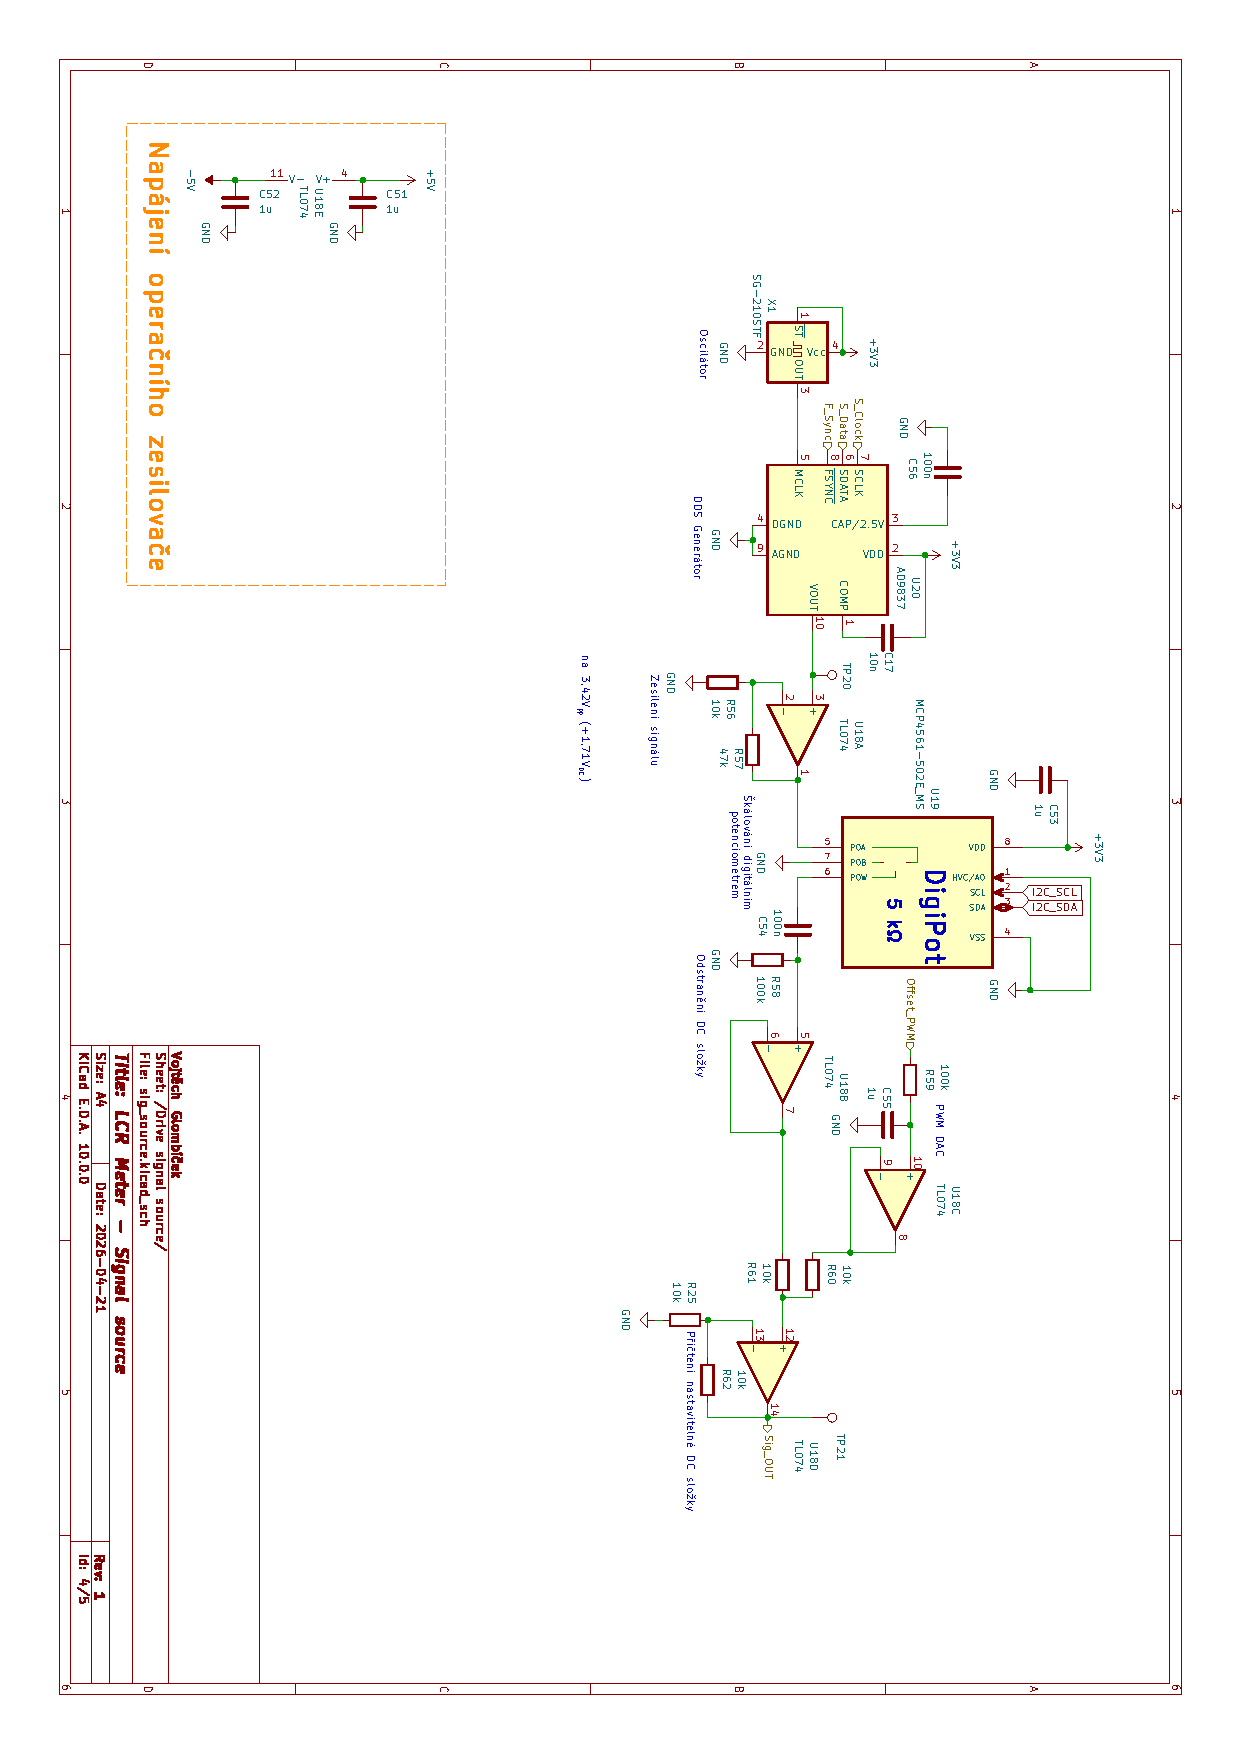
\includegraphics[width=\textwidth,height=\textheight,keepaspectratio]{obrazky/schema+layout/Final_LCR_Meter_page_4.pdf}
    \caption{Schéma -- strana 4 - zdroj měřicího signálu}
\end{figure}

\begin{figure}[H]
    \centering
    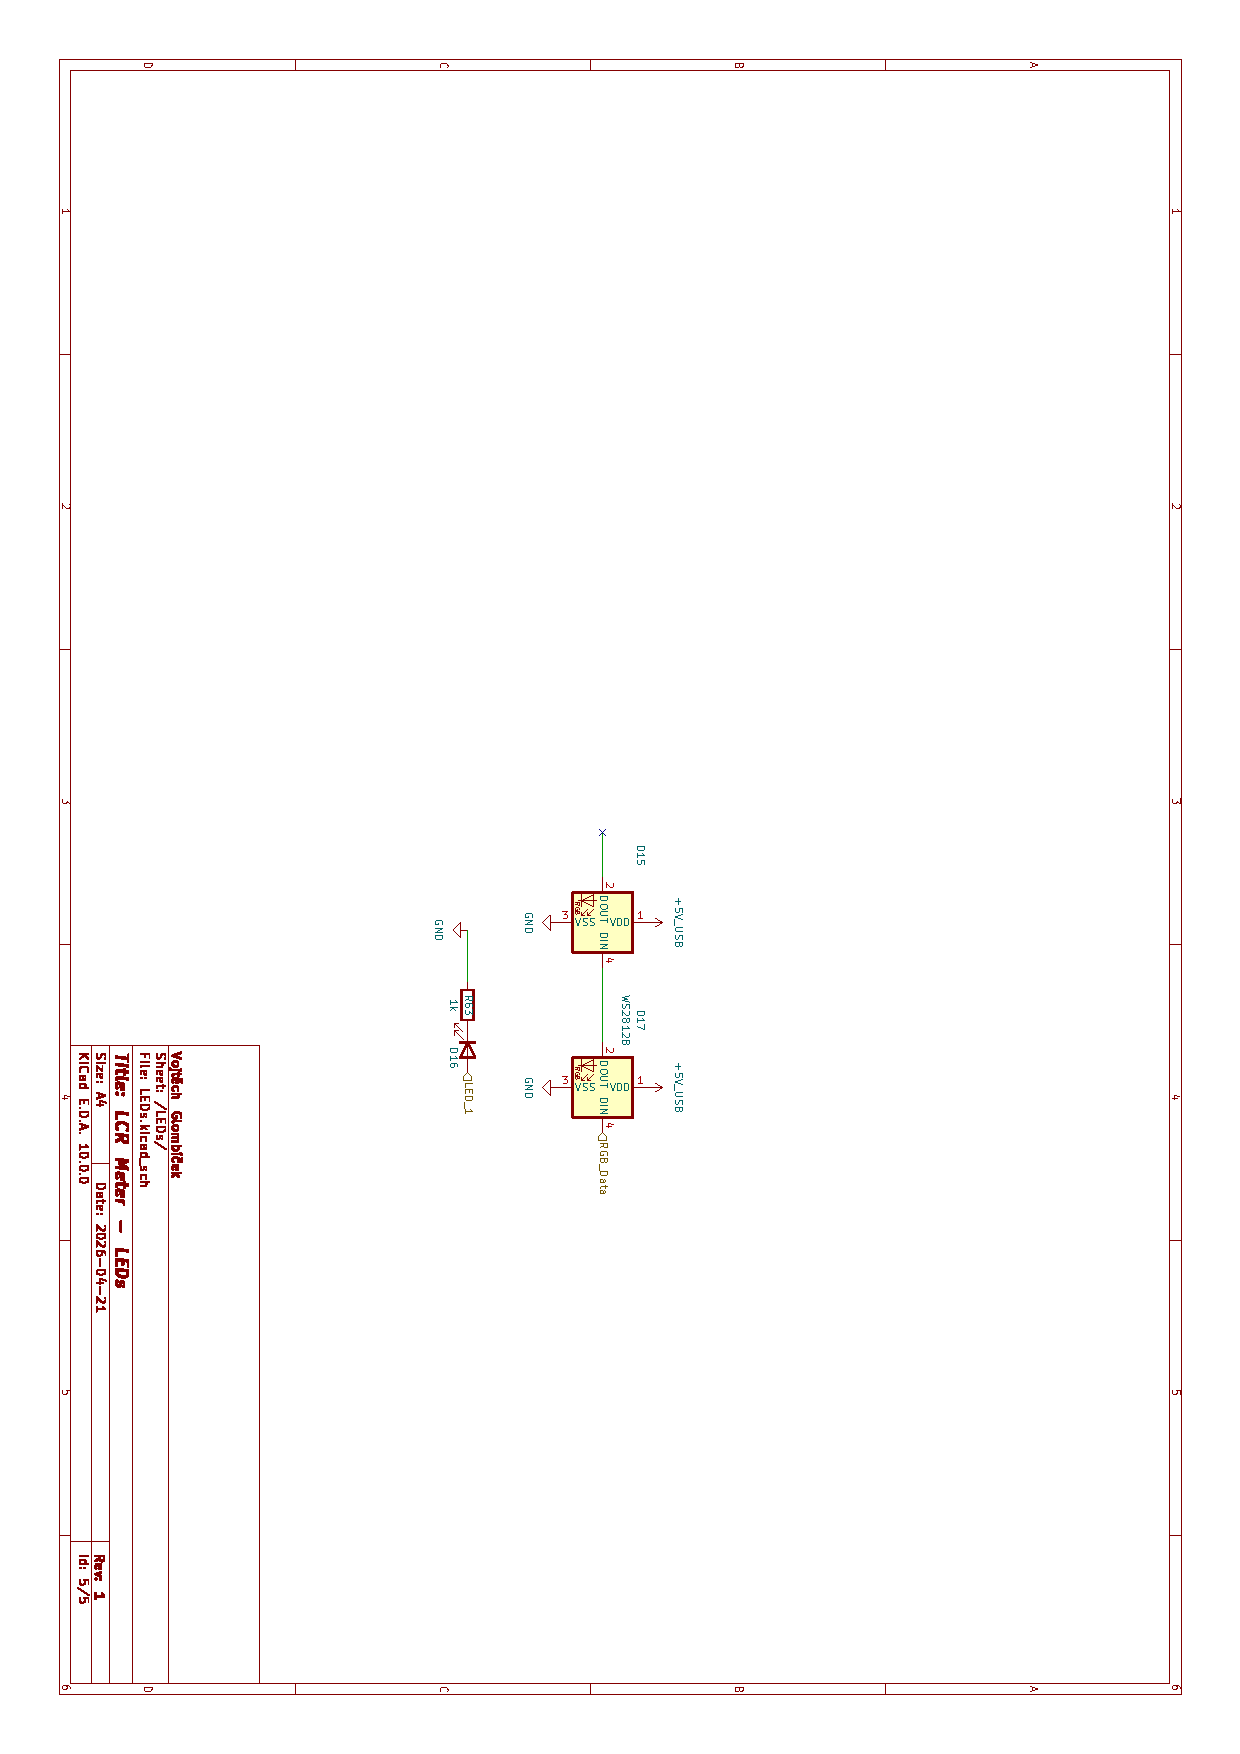
\includegraphics[width=\textwidth,height=\textheight,keepaspectratio]{obrazky/schema+layout/Final_LCR_Meter_page_5.pdf}
    \caption{Schéma -- strana 5 - indikační LED}
\end{figure}

\section{Vodivé motivy DPS}
\label{app:pcb_layers}

\begin{figure}[H]
    \centering
    \begin{minipage}{0.48\textwidth}
        \centering
        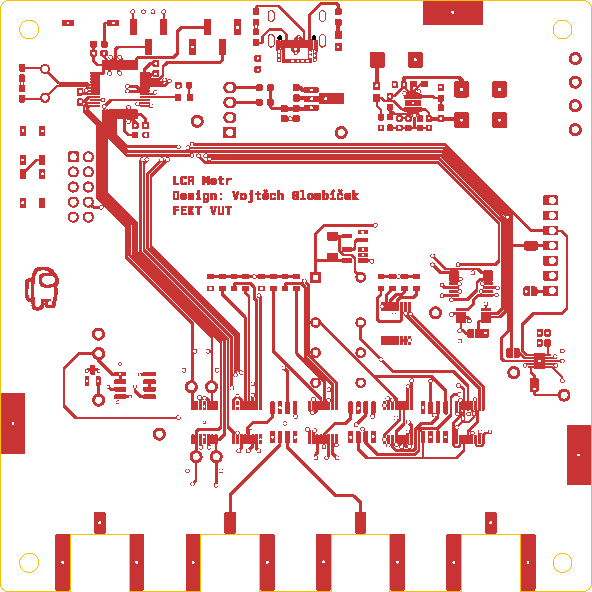
\includegraphics[width=\linewidth,height=0.28\textheight,keepaspectratio]{obrazky/schema+layout/cu_F.pdf}
        \caption{Vrstva Top}
    \end{minipage}
    \hfill
    \begin{minipage}{0.48\textwidth}
        \centering
        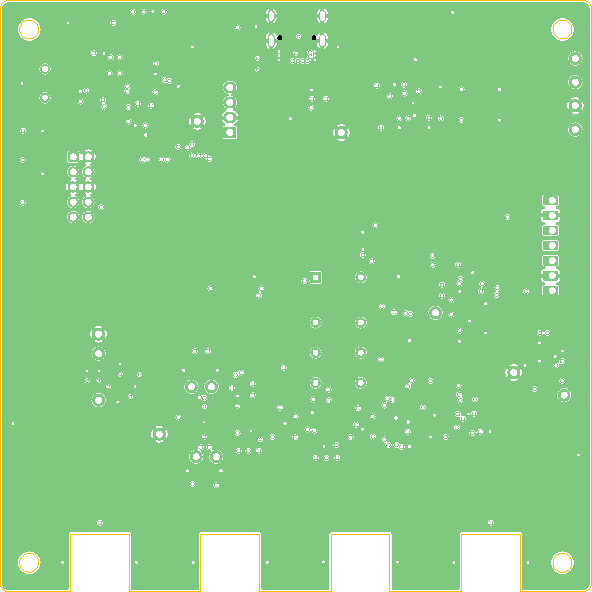
\includegraphics[width=\linewidth,height=0.28\textheight,keepaspectratio]{obrazky/schema+layout/cu_in1.pdf}
        \caption{Vrstva In1}
    \end{minipage}

    \vspace{0.3em}

    \begin{minipage}{0.48\textwidth}
        \centering
        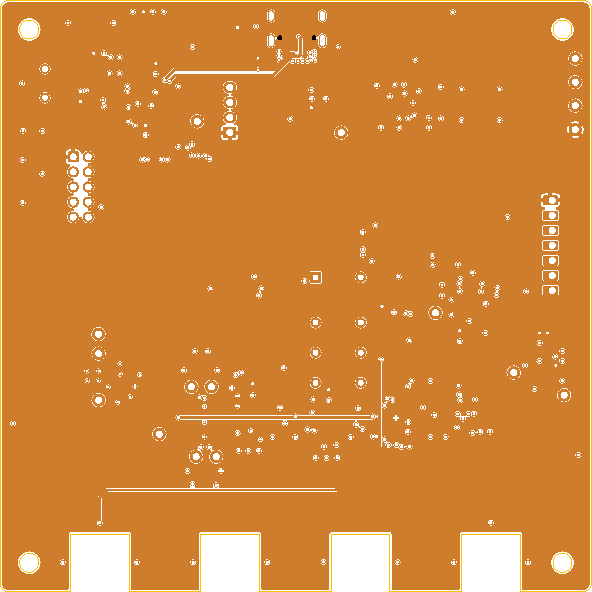
\includegraphics[width=\linewidth,height=0.29\textheight,keepaspectratio]{obrazky/schema+layout/cu_in2.pdf}
        \caption{Vrstva In2}
    \end{minipage}
    \hfill
    \begin{minipage}{0.48\textwidth}
        \centering
        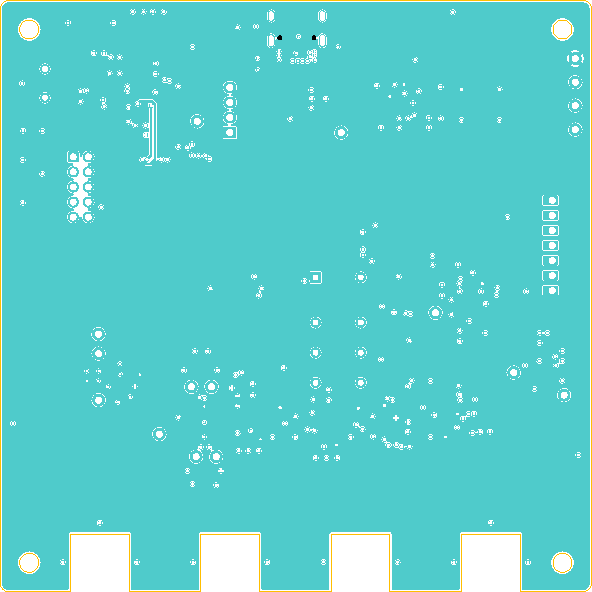
\includegraphics[width=\linewidth,height=0.29\textheight,keepaspectratio]{obrazky/schema+layout/cu_in3.pdf}
        \caption{Vrstva In3}
    \end{minipage}

    \vspace{0.3em}

    \begin{minipage}{0.48\textwidth}
        \centering
        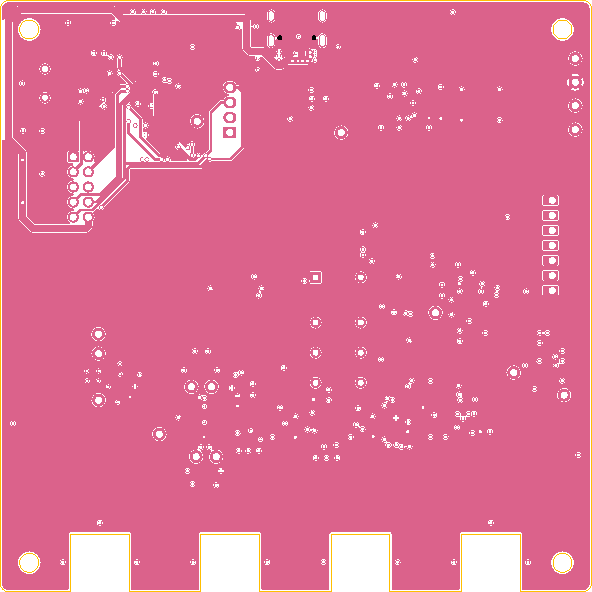
\includegraphics[width=\linewidth,height=0.29\textheight,keepaspectratio]{obrazky/schema+layout/cu_in4.pdf}
        \caption{Vrstva In4}
    \end{minipage}
    \hfill
    \begin{minipage}{0.48\textwidth}
        \centering
        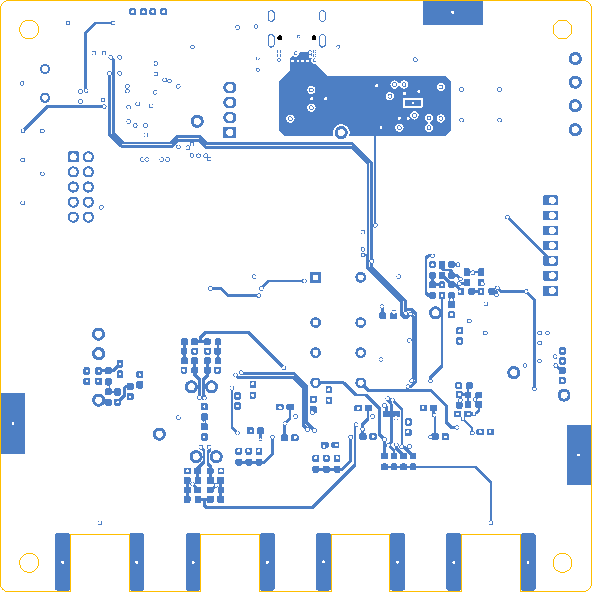
\includegraphics[width=\linewidth,height=0.29\textheight,keepaspectratio]{obrazky/schema+layout/cu_B.pdf}
        \caption{Vrstva Bottom}
    \end{minipage}
\end{figure}

%\restoregeometry


